\documentclass{include/thesisclass}
\usepackage{tabularx}
\usepackage{changepage}
\usepackage{subfig}
\usepackage{float}
\usepackage[outputdir=out]{minted}
\usemintedstyle{pastie}
% \usepackage[printonlyused,withpage]{acronym}
% \usepackage[draft]{showlabels}
% \showlabels{cite}
% \showlabels{gls}
% \showlabels{todo}

\usepackage{csquotes}
\usepackage[acronym,toc]{glossaries}
\setacronymstyle{long-short}
\makeglossaries
\newacronym{LM}{LM}{Language Model}
\newacronym{LLM}{LLM}{Large Language Model}
\newacronym{NER}{NER}{Named Entity Recognition}
\newacronym{ER}{ER}{Entity Recognition}
\newacronym{MOF}{MOF}{Metal Organic Framework}


\newacronym{TF-IDF}{TF-IDF}{Term Frequency - Inverse Document Frequency}
\newacronym{BM25}{BM25}{\todo{explain bm25}}
\newacronym{BERT}{BERT}{Bidirectional Encoder Representation from Transformers}
\newacronym{SOTA}{SOTA}{State of the Art}
\newacronym{NLP}{NLP}{Natural Language Processing}





\newglossaryentry{GPT2}{
    name=GPT2,
    description={The second generation \textbf{G}enerative \textbf{P}retrained \textbf{T}ransformer \gls{LM} from \gls{OpenAI} \cite{radford_language_2019}.}
}

\newglossaryentry{GPT3}{
    name=GPT3,
    description={The third generation \textbf{G}enerative \textbf{P}retrained \textbf{T}ransformer \gls{LM} from \gls{OpenAI} \cite{brown_language_2020}.}
}

\newglossaryentry{GPT4}{
    name=GPT4,
    description={The fourth generation \textbf{G}enerative \textbf{P}retrained \textbf{T}ransformer \gls{LM} from \gls{OpenAI} \cite{openai_gpt4_2023}. Currently their most capable model.}
}

\newglossaryentry{bloom}{
    name=BLOOM,
    description={BigScience Large Open-science Open-access Multilingual Language Model, a 176 billion parameter open-source \gls{LLM} trained on \gls{Google} infrastructure in a concerted effort also including \gls{hf} and other organizations}
}


\newglossaryentry{opt}{
    name=OPT,
    description={Open Pretrained Transformer, a 178 billion parameter open-source \gls{LM} from \gls{Meta} research}
}

\newglossaryentry{Meta}{
    name=Meta,
    description={Previously known as Facebook, Meta regularly open-sources \gls{SOTA} \glspl{LLM}
    }
}

\newglossaryentry{OpenAI}{
    name=OpenAI,
    description={American company at the frontier of scaling deep learning architectures. Models that pushed boundaries include \glspl{LM} such as \gls{GPT2}, \gls{GPT3} and \gls{GPT4} as well as image generation models}
}

\newglossaryentry{Google}{
    name=Google,
    description={Search Engine giant}
}

\newglossaryentry{hf}{
    name=HuggingFace,
    description={American deep learning ecosystem Startup}
}


\interfootnotelinepenalty=10000

\newcommand{\vect}[1]{\boldsymbol{\bm{#1}}} % for package bm

\SelectLanguage{english}
% details on this thesis
\newcommand{\thesisauthor}{Felix Karg}
%\newcommand{\thesistopic}{Name des Themas auf Deutsch}

%\newcommand{\thesisentopic}{Extraction of structural information from powder X-ray diffraction patterns
%using neural network based on randomly generated crystals}
%\newcommand{\thesisentopic}{Analysis of Powder X-Ray Diffractograms
%Using Neural Networks Trained on an Infinite Stream of Synthetic Patterns}
%\newcommand{\thesisentopic}{Analysis of Powder X-Ray Diffractograms
%Using Neural Networks Trained on Continuously Generated Synthetic Patterns}
%\newcommand{\thesisentopic}{Analysis of Powder X-ray Diffractograms Using Neural Networks Based on
%Synthetic Patterns Generated During Training}
%\newcommand{\thesisentopic}{Analysis of Powder X-Ray Diffractograms
%Using Neural Networks Trained on Continuously Generated Synthetic Patterns}
\newcommand{\thesisentopic}{A Benchmark on Using Large Language Models for Zero-Shot Automated Data Extraction from Scientific Literature}

\newcommand{\thesisinstitute}{Institute of Theoretical Informatics}
\newcommand{\thesisreviewerone}{T.T.-Prof. Dr. Pascal Friederich}
\newcommand{\thesisreviewertwo}{Prof. Dr. Second Reviewer}
\newcommand{\thesisadvisorone}{Tobias Schlöder}
\newcommand{\thesistimestart}{2023-03-01} % on titlepage
\newcommand{\longdate}{2nd October 2023} % on signature lines
\newcommand{\thesistimeend}{2023-10-02} % on titlepage
\newcommand{\thesistimehandin}{2023-10-02} % on second page 'preamble'
\newcommand{\thesispagehead}{\thesisentopic} % page heading


% ----------------- referencing ----------------
\newcommand{\secref}[1]{Section~\ref{sec:#1}}
\renewcommand{\subref}[1]{Subsection~\ref{sub:#1}}
\newcommand{\chapref}[1]{Chapter~\ref{chap:#1}}
\renewcommand{\eqref}[1]{Equation~(\ref{eq:#1})}
\newcommand{\figref}[1]{Figure~\ref{fig:#1}}
\newcommand{\tabref}[1]{Table~\ref{tab:#1}}
\newcommand{\coderef}[1]{Code Example~\ref{code:#1}}
\newcommand{\outref}[1]{Output~\ref{out:#1}}

\newcounter{code}
\setcounter{code}{0}
\newenvironment{codeboxed}[2]{
    \begin{minipage}{\linewidth}\begin{center}\textbf{#1}\\\small #2\\[1ex]\begin{tabular}{|p{\textwidth}|}\hline}{
    \\\hline\end{tabular}\end{center}\end{minipage}}

\newcommand{\code}[3]{\refstepcounter{code}\label{code:#2}\begin{codeboxed}{Code Example \thecode}{#3}
        \inputminted[linenos,fontsize=\small]{Python}{code/#1}\end{codeboxed}}


\hypersetup
{
    pdfauthor={\thesisauthor},
    pdftitle={\thesisentopic},
    pdfkeywords={kit,informatics,master,thesis,\thesisauthor}
}

% Describe separation hints here:
\hyphenation
{
    über-nom-me-nen an-ge-ge-be-nen
}

\addbibresource{references.bib}


\begin{document}

% Always use the primary source of information (probably mostly relevant in introduction)
% Referencing whole paragraph after full stop is fine (Harvard style).
% ~ is an unbreakable space.

% Punctuation for equations:
% - Use "equation" blocks
% - Use \,. to set a point after an equation.
% See: https://tex.stackexchange.com/questions/7542/for-formal-articles-should-a-displayed-equation-be-followed-by-a-punctuation-to

% Page numbers required for direct quotations.
% Can also be helpful for indirect quotations, for example to locate the source in a big book etc.
% For papers not necessary.

% Cite entire paragraph after final period: https://tu-dresden.de/bu/umwelt/geo/ifk/ressourcen/dateien/downloads/TUM-Citation-Guide.pdf?lang=de

\newcommand{\diameter}{20}
\newcommand{\xone}{-15}
\newcommand{\xtwo}{160}
\newcommand{\yone}{15}
\newcommand{\ytwo}{-253}

\fancypagestyle{alim}{\fancyhf{}\renewcommand{\headrulewidth}{0pt}
	\fancyfoot[R]{\footnotesize{\textbf{www.kit.edu}}}
	\fancyfoot[L]{\footnotesize{KIT – The Research University in the Helmholtz Association}}
}

\begin{titlepage}

	\thispagestyle{alim}

	\noindent
	% KIT image and sign for faculty of physics

	\noindent\begin{minipage}{0.25\textwidth}% adapt widths of minipages to your needs
		
\includegraphics[width=1\textwidth]{include/kitlogo.pdf}
	\end{minipage}
	\hfill
	\begin{minipage}{0.25\textwidth}\raggedleft
		
\includegraphics[width=1\textwidth]{include/AiMat_logo_purple.png}
	\end{minipage}

    \centering

    % thesis topic (en and ge)
	\vspace*{4.0cm}

	\large\par\noindent\rule{\textwidth}{1.2pt}

	\Huge \thesisentopic

	\large\par\noindent\rule{\textwidth}{1.2pt}

    % author name and institute
    \vspace*{2cm}
    \Large Master thesis\\by\\
    \vspace*{1cm}
    \huge\thesisauthor\\
    \vspace*{1cm}
    \Large \thesisinstitute

    % examiners (Referenten)
    \vspace*{4cm}
    \large
    \begin{center}
        \begin{tabular}[ht]{l c l}
        \iflanguage{english}{Reviewer}{Referent}: 
            & \hfill & \thesisreviewerone\\
        \iflanguage{english}{Second Reviewer}{Korreferent}: 
			& \hfill & \thesisreviewertwo\\
        \iflanguage{english}{Advisor}{Betreuender Mitarbeiter}: 
            & \hfill & \thesisadvisorone\\ \\
        % uncomment if you want to provide info on more than one advisor
        %\iflanguage{english}{Second Advisor}{Zweiter betreuender Mitarbeiter}: 
        %    & \hfill & \thesisadvisortwo\\
		\large{Begin:}
			& \hfill & \large{\thesistimestart}\\
			\large{Submission:}
            & \hfill & \large{\thesistimeend}\\
        \end{tabular}
    \end{center}

\end{titlepage}

\chapter{Acknowledgements}

\todo{say thanks to anyone who gave you support while you worked on your thesis/dissertation. Many people use this section to give credit to their advisor, editor, or even their parents. If you received any funding for your research or technical assistance, make sure to mention it here.}


\begin{itemize}
    \item supervisors
    \item family
    \item friends
    \item proofreaders
    \item university
    \item hpc shoutout
    \item whomever else
\end{itemize}

\chapter*{Declaration of Authorship}

Find the appropriate and up-to-date text in your Studienordnung and copy it here.\\

\vspace{1cm}

\noindent Karlsruhe, Month dd, yyyy \hfill \parbox[t]{.5\linewidth}{\rule[-3pt]{\linewidth}{.4pt}\par\smallskip
    \centering Your name}

\vfill

Approved as examination copy:\\

\vspace{1cm}

\noindent Karlsruhe, Month dd, yyyy \hfill \parbox[t]{.5\linewidth}{\rule[-3pt]{\linewidth}{.4pt}\par\smallskip
    \centering}

\renewcommand{\arraystretch}{1}

\cleardoublepage

\pagenumbering{Roman}
\renewcommand{\cftchapfont}{%
    \bfseries
}

\tableofcontents                    % listoftables on new pages
\begingroup \let\clearpage\relax    % in order to avoid listoffigures and
\newpage
\listoffigures
% \newpage
% \listoftables
\endgroup
\cleardoublepage

% Contents
\MainMatter

\addchap{Abstract}\label{chap:abstract}
\pagenumbering{arabic}

% How to write an abstract
%  One or two sentences providing a basic
%  introduction to the field, comprehensible to
%  a scientist in any discipline.
A majority of materials science knowledge is contained in unstructered text scattered throughout the body of scientific literature, out of reach for increasingly capable but data-starved \acrlong{ML} models that are being used more and more at every step of the materials creation process.
%  Two to three sentences of more detailed
%  background, comprehensible to scientists
%  in related disciplines.
Thus, the extraction of such information from unstructured scientific literature and conversion to machine-readable formats has become a challenge of \acrlong{NLP}.
Recently, \acrlongpl{LLM} have gained prominence for their general capabilities across \acrlong{NLP} tasks, including \acrlong{NER}.
%  One sentence clearly stating the general
%  problem being addressed by this particular
%  study.
%However, such information is often not accessible in a machine-readable format.
%  One sentence summarizing the main result
%  (with the words “here we show” or their
%  equivalent).
This work demonstrates that automated information extraction from materials science literature is possible with high accuracy using models of only 13 billion parameters and without fine-tuning.
%  Two or three sentences explaining what the
%  main result reveals in direct comparison to
%  what was thought to be the case previously,
%  or how the main result adds to previous
%  knowledge.
In fact, 13 billion parameter sized variants from both \model{llama} and \model{llama2} achieved an accuracy of 95 to 98\% for the extraction of temperature and time information from unstructured text.
Additionally, the 7 billion parameter sized \model{falcon} achieved an accuracy of 79\% on the extraction of solvent information from synthesis paragraphs on the creation of \acrlongpl{MOF}.
%Contrary to expectation, fine-tuning is harder than expected with few resources available.
%  One or two sentences to put the results
%  into a more general context.
The smaller size of these models, their open-access availability, and no necessity for additional fine-tuning enables the usage of most consumer hardware, making these capabilities far more accessible than previously expected.
%  Two or three sentences to provide a broader
%  perspective, readily comprehensible to a
%  scientist in any discipline.

% This means, that even for more sophisticated information extraction tasks fine-tuning might not be necessary, particularly with more generally capable models in the future.

\addchap{Zusammenfassung}
Deutsche Zusammenfassung hier. \todo{write zusammenfassung}


\cleardoublepage
% \pagenumbering{arabic}
% other page numbering styles:
% - arabic: use Arabic numerals (1, 2, 3, ...)
% - alph: use lowercase letters (a, b, c, ...)
% - Alph: use uppercase letters (A, B, C, ...)
% - roman: use lowercase roman numerals (i, ii, iii, ...)
% - Roman: use uppercase roman numerals (I, II, III, ...)




\chapter{Introduction}\label{chap:introduction}

% clear and concise:
%  Presentation of the topic and the background
Unstructured scientific literature contains a vast amount of materials science knowledge, and is the only place to get it.
However, this places it squarely out of reach for further processing, which makes it difficult or impossible to build on a large part of prior work.
%  Motivation of importance
\gls{ML} models are increasingly used in screening steps for materials discovery and property prediction \cite{saal_machine_2020, luo_mof_2022, choudhary_recent_2022}, among other steps.
% These models continue to get better, but often the biggest bottleneck is a lack of data.
In general, more high-quality data improves the output quality of \gls{ML} models considerably \cite{hoffmann_empirical_2022}.
%  Research gap, research question
Currently, the amount of data accessible to train such models is limited, \todo{@Tobias check} in particular from older or less known work.

Over the last year, \glspl{LLM} rose to public prominence since the launch of \gls{ChatGPT}.
Regardless of public perception, recent improvements across \gls{NLP} benchmarks are undeniable \cite{devlin_bert_2018, openai_gpt4_2023}.
In this work, \glspl{LLM} are used for information extraction of scientific text on synthesisizing \glspl{MOF}.

% Structure of the thesis
\draft{
Structure.
}
% Short summary of main results
\draft{
Results summary.
}

% \section{Motivation}
% Take for example the field of synthesizing Metal-Organic Frameworks (MOFs)
% \cite{zhou_introduction_2012}. While numerous detailed descriptions of
% synthesis procedures exist, they are not available in machine-readable formats,
% which prevents effective application of state-of-the-art techniques such as
% automated experimentation \cite{shi_automated_2021} or synthesis parameter prediction
% \cite{luo_mof_2022}. Thus, we intend to create a pipeline for deriving
% machine-readable information on MOF synthesis parameters from given questions
% on provided scientific articles.

% Motivation
% \begin{itemize}
%     \item vast amount of material science knowledge scattered across papers
%     \item often non-machine readable formats
%     \item makes it difficult or impossible to build on (all) prior work
%     \item results in tremendous duplicates and other unnecessary work
%     \item a lot of insights to be gained from such a database, as well as automated experimental design (and possibly execution)
% \end{itemize}


\section{Scientific Question}\label{sec:question}

The goals of this work are threefold:
\begin{enumerate}
    \item Demonstrate zero-shot automated information extraction from scientific literature using open-access \glspl{LLM}.
    \item Benchmark and compare the accuracy of currently available open-access \glspl{LLM} for the automated information extraction from scientific literature.
    \item Attempt fine-tuning of open-access \glspl{LLM} in order to increase accuracy.
\end{enumerate}

As part of this work, a highly flexible automated pipeline for the extraction of non-machine readable information in \gls{MOF} synthesis will be created.
The approach chosen in this work will be discussed in more detail \chapref{approach}, where the implementation is described in \secref{impl}, the models used in \secref{models}, and \secref{data} describes the source of data.


\newpage
collection of todos
\todo{find a first section for introduction chapter}

explain stuff somewhere
\todo{explain context length somewhere}
\todo{explain zero-shot somewhere}
\todo{explain causal and masked language models somewhere}

\chapter{Background}\label{chap:background}
\todo{write background}
Core meta points:
\begin{itemize}
    \item up to five pages background
    \item go from very general to very related to topic, end with questions to resolve
\end{itemize}

\section{General Work, Related}\label{sec:general}
\todo{think about it if I actually want to include this section}
ml models increasingly used in screening steps for materials discovery and property prediction
% “Machine learning in materials discovery: Confirmed predictions and their underlying approaches"
% “Recent advances and applications of deep learning methods in materials science"

\section{Related Work}\label{sec:related}
% \todo{write section}
\todo{related work is only entity recognition stuff}

\subsection{Rule-Based Entity Recognition}\label{sub:ER}
There have long been rule-based approaches for the recognition of individual
entities (e.g. Temperature). ChemTagger \cite{hawizy_chemicaltagger_2011}
and others \cite{beard_comparative_2019, huang_database_2020}
clearly demonstrated that simple rule-based systems can sometimes extract much
of the requested information. They can often
achieve high precision for simple, well-defined
tasks, but tend to be highly specialized and
are hard to adapt to differing circumstances.

\todo{establish ER and NER}



\todo{Notes from Jehona Talk, adapt accordingly}
\begin{itemize}
    \item Techniques like TF-IDF or BM25 ??
    \item 'it is called extractive because it extracts the answer from a agiven
        context, rather than generating a new answer'
    \item using haystack as llm framework
    \item using a document store and memorizing architecture? dense retrieval:
        'using dense embeddings rather than sparse ones'
    \item
\end{itemize}

\paragraph{BM25}

\gls{BM25} is a ranking function that ranks a set of documents based on the query terms appearing in each document, regardless of the inter-relationship between the query terms within a document (e.g., their relative proximity).

\paragraph{TF-IDF}
\gls{TF-IDF} is a handy algorithm that uses the frequency of words to determine how relevant those words are to a given document.

\section{Language Models for Data Extraction Tasks}
\todo{write lms for data extraction and then move it to background}
It was shown that fine-tuning \gls{BERT} for \gls{NER} tasks in materials science has good results \cite{zhao_finetuning_2021}.

\subsection{Using LLMs for Data Extraction}
Fine-tuning \gls{GPT3} with 100 manual and 500 partially augmented examples of data extraction
created one of the most sophisticated pipelines for information extraction \cite{dunn_structured_2022}.
Most of our work will be similar to theirs. However,
Chinchilla \cite{hoffmann_training_2022} and CoTR \cite{zhang_multimodal_2023}
demonstrated that while achieving impressive capability, such large models are
substantially overparametrized and undertrained. Additionally, while the
results are state-of-the-art, GPT3 is only accessible through the API of
OpenAI, a for-profit company. This considerably limits access to model
internals.

Our work differs from \cite{dunn_structured_2022} by addressing these two
caveats. Instead of GPT3, we use a similarly capable open-source model called
OPT \cite{zhang_opt_2022}. Self-hosting enables us to do deep introspection
necessary for state-of-the-art prompt engineering and gives us the required
freedom to attempt distillation \cite{sun_patient_2019}, which addresses
overparametrization. Distillation promises substantial model parameter
reduction with little loss in accuracy (50x parameter reduction while keeping
95\% accuracy), and has been confirmed to have similar compression characteristics
for other large language models.
\todo{rewrite section on LLMs}




\newpage
\section{Scientific Question}\label{sec:question}
\todo{expand scientific question}

how well can we automate the extraction of parameters from scientific data using \glspl{LLM} with zero-shot

The goal of this work is to benchmark the accuracy of open source \glspl{LLM} to
demonstrate automated extraction of unstructured text from scientific
literature and create an automated pipeline for the creation of a database with otherwise non-machine readable information on \gls{MOF} synthesis or similar tasks.

% By
% doing so, we create a training pipeline that can be a) self-hosted and b)
% adapted to other data extraction tasks. It may be provided as a service for
% other research groups.
%
% In this work, we will use OPT \cite{zhang_opt_2022} to empirically test how
% much accuracy can be improved via 1) fine-tuning and 2) prompt engineering.
% Additionally, we intend to 3) test how accuracy and compute requirements will be
% affected by reduction of model size via distillation \cite{sun_patient_2019}.
% A reduction in parameters would make it considerably less compute intensive to
% run the final model.

\chapter{Methods}\label{chap:methods}
% Evaluation Criteria:
% - Explanation
% - Reproducibility
% - Visualization
\todo{write methods introduction}
{\color{blue}
Chapter on tools (language models) used. What exactly do I want to explain?
First, a bit on how they work in general, second a bit of background on the models, a bit of a comparison (architecture and benchmarks?)
}

% background is more general, methods is specific to the methods we use, in our case LLMs

\section{Language Model Basics}\label{sec:basics}
This Section aims to provide an overview and fundamental understanding of the underlying concepts and terminology of the language models used in this work.
The models part of the benchmark are introduced in \secref{models}.
We will first establish the fundamentals of the transformer architecture in \subref{transformer} and take a look at the development to a \acrlong{LLM} in \subref{llm} before combining a number of common adaptions to visualize how a modern transformer architecture often looks like in \subref{modern}.
\todo{rewrite methods basics referecing when the other parts are finished}

\begin{figure}[!htb]
    \begin{centering}
        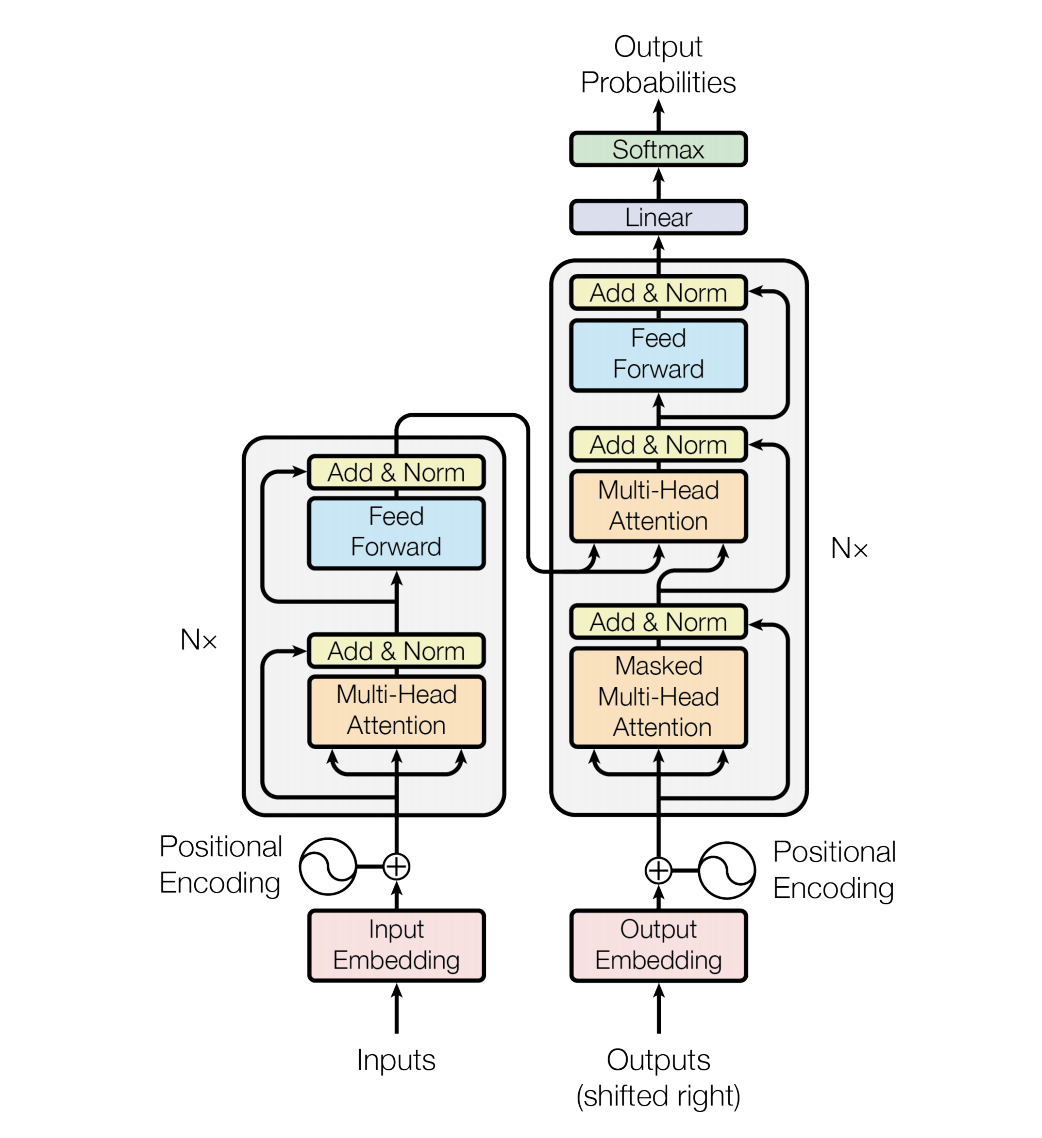
\includegraphics[height=0.5\textheight]{img/transformer}
        \caption[Original Transformer Architecture]{\textbf{Original Transformer Architecture.}
        The architecture was originally conceptualized for translation between languages.
        For that effect the text to translate (input) will be fully encoded to the embedding space, added to a positional encoding, and passed through alternating layers of self-attention and \gls{MLP} feed-forward layers with \gls{ReLU} activation, with residual connections and normalization after each.
        Output is generated autoregressively (generating each output token one-by-one, and append it to outputs to generate the next one), and has an additional layer of cross-attention to the input embedding.
        \Glspl{causal} are exclusively autoregressive decoder-only models.
        % The text to translate \textit{from} is the input, and the model will autoregressively (append selected output token to the outputs to generate the next output token until the full output has been generated) generate the full output.
        Image Source: \cite{vaswani_attention_2017}
        }
        \label{fig:transformer}
    \end{centering}
\end{figure}

% \begin{figure}[!htbp]
%     \begin{centering}
%         \subfloat[Runtime in minutes for correcting 25kb Matrix]
%         {\includegraphics[scale=0.9]{figures/results/runtime_25}} \\
%         % \caption[Correction time of 25kb]
%         % {\textbf{Runtime in minutes} for correcting the 25kb matrix.}
%         \subfloat[Runtime in minutes for correcting 50kb Matrix]
%         {\includegraphics[scale=0.9]{figures/results/runtime_50}}
%         \caption[Algorithm Runtimes]
%         {\textbf{Algorithm Runtimes} for correcting the different matrices. It
%         remains an open question why the difference between KR and RUST stays the
%         same, even though both ICE and RUST double their computation time. Smaller
%         is better.}
%         \label{fig:transformer}
%     \end{centering}
% \end{figure}


\subsection{The Transformer Architecture}\label{sub:transformer}
All modern language models are based on what Google introduced as the transformer architecture \cite{vaswani_attention_2017}. 
This architecture originally consisted of an encoder and a decoder (See \figref{transformer} for more details).
This new transformer architecture quickly established itself by outperforming other architectures available at the time with a fraction of the training cost.
An Encoder-Only transformer architecture, specifically \gls{BERT} set a new \gls{SOTA} for all \gls{NLP} benchmarks established at the time.
% This success was not limited to \gls{NLP} tasks.

% Along with significantly increasing capability in \acrlong{NLP}, these models enabled more sophisticated requests for data extraction.

% main difference to before: enabled more context compared to LSTM-based attention stuff (andscaling)

\subsection{A Modern Transformer Architecture}\label{sub:modern}

There have been various attempts at improving the transformer architecture \cite{shazeer_glu_2020, su_roformer_2022, ainslie_gqa_2023, bolya_hydra_2022, sukhbaatar_adaptive_2019, lu_understanding_2019, ye_understanding_2023, wu_memorizing_2022}, some of them more successful than others.
When setting up a new transformer model, there are a few established improvements that are used with few exceptions.
Compare with \figref{modern_transformer} for a graphic representation.

As activation functions, early transformer architectures used \gls{ReLU}, but when comparing different activation functions, \gls{SwiGLU} \cite{shazeer_glu_2020} empirically work best for most situations.

Instead of the previous sinusoidal positional encoding, using \gls{RoPE} works a lot better \cite{su_roformer_2022}. So does RMSNorm as LayerNorm \cite{ba_layer_2016}, when using it before instead of after each layer.

Grouping some of the query heads for \gls{GQA} \cite{ainslie_gqa_2023} work better than no sharing or full individual heads \cite{bolya_hydra_2022}.

\begin{figure}[!htbp]
    \begin{centering}
        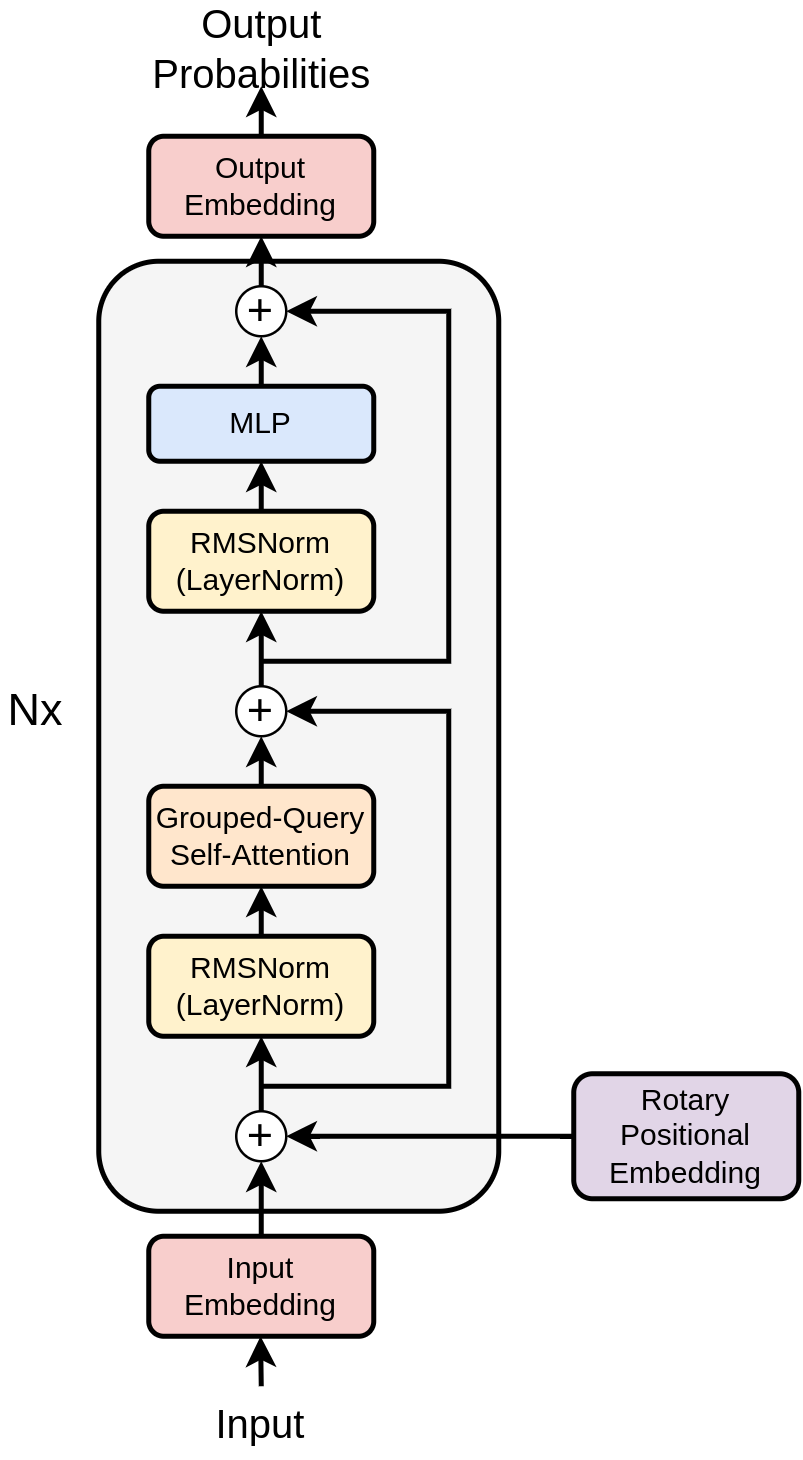
\includegraphics[height=0.8\textheight]{img/modern_transformer}
        \caption[Example of a Modern Transformer Architecture]{\textbf{Example of a Modern Transformer Architecture.} There are a number of differences when compared to the original architecture as seen previously in \figref{transformer}: layers are normalizing the residual with RMSNorm instead of having a normalized residual. Multi-head attention got replaced with \gls{GQA}, and sinusoidal positional embeddings with embeddings from \gls{RoPE} {\em on each layer}. Additionally, activation functions in the \gls{MLP} changed from \gls{ReLU} to \gls{SwiGLU}.}
        \label{fig:modern_transformer}
    \end{centering}
\end{figure}



This architecture, as described here and visualized in \figref{modern_transformer}, is shared with small variations by the \glspl{LLM} introduced later in \secref{models}.
Apart from \model{llama2}, most other \glspl{LLM} do not use \gls{GQA}.

\subsection{Large Language Models}\label{sub:llm}

\gls{GPT2} \cite{radford_language_2019} is a very straightforward transformer architecture, but scaled up more than previous models.
The biggest \gls{GPT2} variant had 1.5 billion parameters, which is 15x more parameters than the biggest \gls{BERT} variant had.
It mainly demonstrated that bigger \glspl{LM} get more capable in general -- and seemingly without limit.

Models with more than a few billion parameters became generally referred to as a \acrlong{LLM}. \gls{GPT3}, the first such model with 176 billion parameters was introduced by \gls{OpenAI} in 2020 \cite{brown_language_2020}.
\glspl{LLM} differ from previous models in both parameter count (usually many billions) and substantial advances in general capability.
These models tend to have smaller siblings of the same architecture with fewer parameters, commonly in th steps of 7 billion, 13 billion, 30 billion, and 70 billion, though availability and exact parameter count varies.
Other Organisations trained \glspl{LLM} of this generation as well, some of them open-source, which demonstrated similar capabilities.
The most well-known models of this wave were \model{BLOOM} and \model{OPT} (throughout 2022).

The most recent and most capable generation of \glspl{LM} got introduced starting early 2023, after the release of \gls{ChatGPT} sparked worldwide interest in \glspl{LLM}. Progress happened fast and many incorporated numerous of the collectively found possible improvements. \glspl{LLM} of this generation are mostly classified so by their capability, and less so through parameter size, albeit their parameter counts still tend to be in the dozens of billions. Models of this category include the open-source \model{llama} and its well-known derivatives \model{alpaca} and \model{vicuna}, \model{falcon}, as well as most recently \model{llama2}.

For more details on most of the aforementioned models, see \secref{models}.


\section{Training Large Language Models}\label{sec:training}
\todo{write section on training methods}

\subsection{Pretraining}\label{sub:pretraining}
for main training usually crossentropy loss on text, decent batchsizes, large scale distributed.
\todo{write subsection on pretraining}

\subsection{Fine-Tuning}\label{sub:finetune}
specialized, mostly task-specific training making use of transfer-learning from a generalized model, making them capable for tasks where not much data is available
\todo{write subsection on finetuning}

\subsection{Fine-Tuning on Instructions}\label{sub:instruct}
mostly just changing 'expectation distribution' of model, giving preferred answers when interacting with the model for most people

a model fine-tuned on a instruction dataset or setting is commonly referred to as a 'instruct'-variant.
\todo{write subsection on instruction-finetuning}

% \subsection{RLHF}\label{sub:rlhf}
% learning preference policy to later fine-tune the large model on. basically lobotomization, as it drastically reduces capability.
% Well, write it a bit nicer than that.
% \todo{this is not really relevant for my thesis. remove? or write?}

\chapter{Approach}\label{chap:approach}
Chapter on {\em how} I used the language models, what I tried, and what didn't work / I settled on.

See \subref{list} for a list of the models used, \subref{criteria} for selection criteria and the respective Subsection for more details on each model.

\section{Prompts}\label{sec:prompts}

used a form of guidance \cite{guidance_2023}

\section{Supervised Fine Tuning}\label{sec:sft}
Was attempted multiple ways, utterly failed

How much should I write about?

curiousity with \verb`input_ids` and \verb`labels`? resulted in broken model, probably learned that it's 'finished', only outputting EOS tokens. Not sure if doing this otherwise would actually change anything though

Attempts at mask manipulation: not possible with causalLMs (they are all of this type)

SFT: only published about 1months before deadline, a lot of magic that isn't documented properly, at all. Couldn't get it to run, gave up due to time limit.

\section{Comparison}
criteria for comparing the outputs with labels

\section{Results}

\begin{frame}[c,fragile,allowframebreaks]{Accuracy Overview}
    \pause
    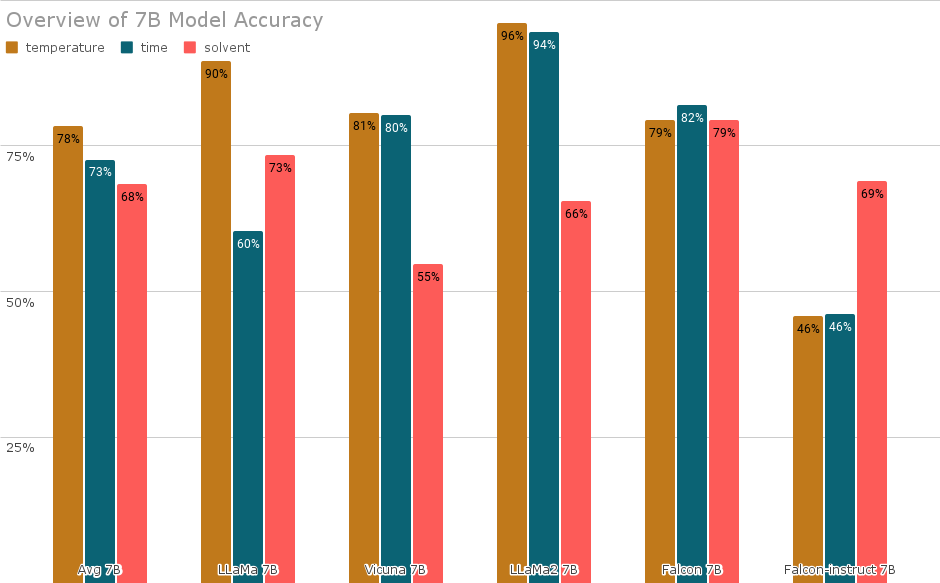
\includegraphics[height=0.7\textheight]{overview_7b_accuracy}
    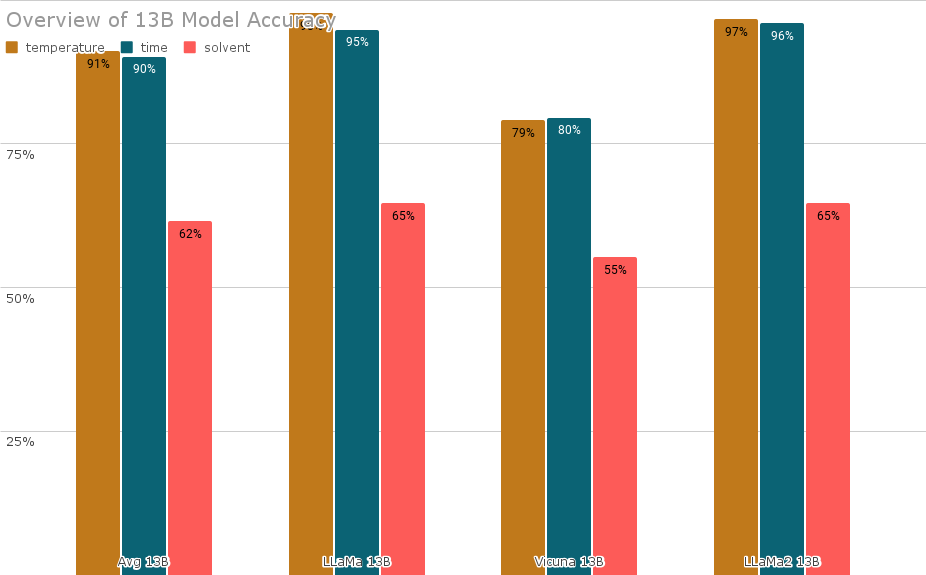
\includegraphics[height=0.7\textheight]{overview_13b_accuracy}
    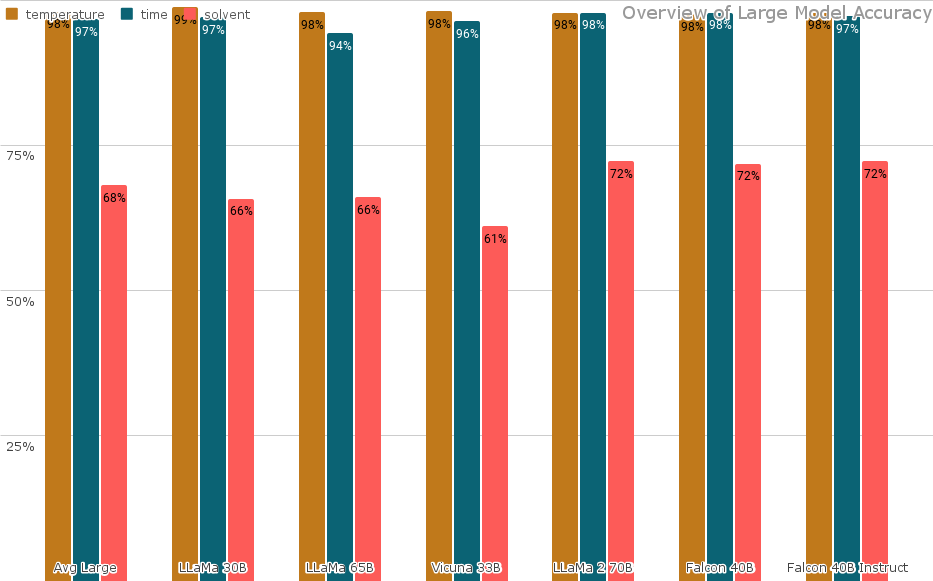
\includegraphics[height=0.7\textheight]{overview_large_accuracy}
\end{frame}



\begin{frame}<handout>[c]{Note on Interesting Outliers}
    \begin{columns}
        \column{0.3\textwidth}
    7B
    \begin{itemize}
        \item \gls{llama}-7B accuracy on \ttemp and \ttime vary substantially across models, but are mostly similar within one model
        \item \tsolv accuracy of \gls{vicuna} bad somehow
        \item Bad \ttemp and \ttime accuracy of \gls{falcon}-instruct
        \item Decent performance from \gls{llama2} overall
    \end{itemize}
        \column{0.3\textwidth}
        \large
        13B
        \begin{itemize}
            \item \gls{vicuna} still lagging behind, though while \gls{falcon} does not have a 13B variant, it should still be worse
            \item Accuracy on \tsolv seems to have gotten worse, on average and for individual models
        \end{itemize}
        \column{0.3\textwidth}
        \large
        30B+
        \begin{itemize}
            \item Average Accuracy very high
            \item \tsolv accuracy only 72\% though, that was higher in 7B models!
        \end{itemize}
    \end{columns}
\end{frame}

\subsection{Frequent Mistakes}

\begin{frame}[c,fragile,allowframebreaks]{Unit Confusion}
    \pause
    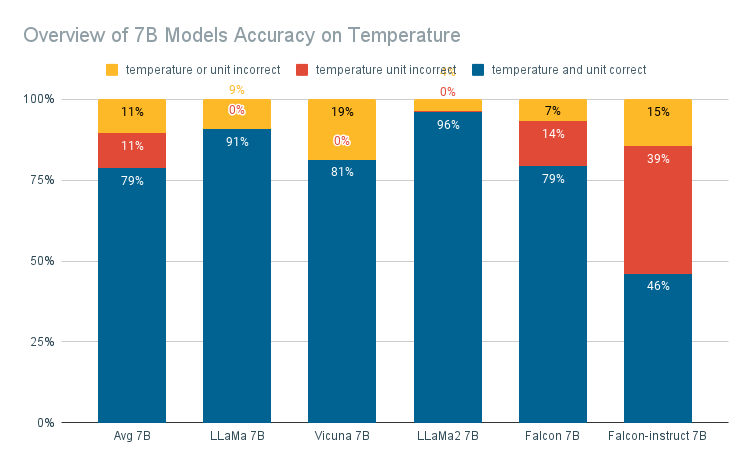
\includegraphics[height=0.7\textheight]{overview_7b_temp}
    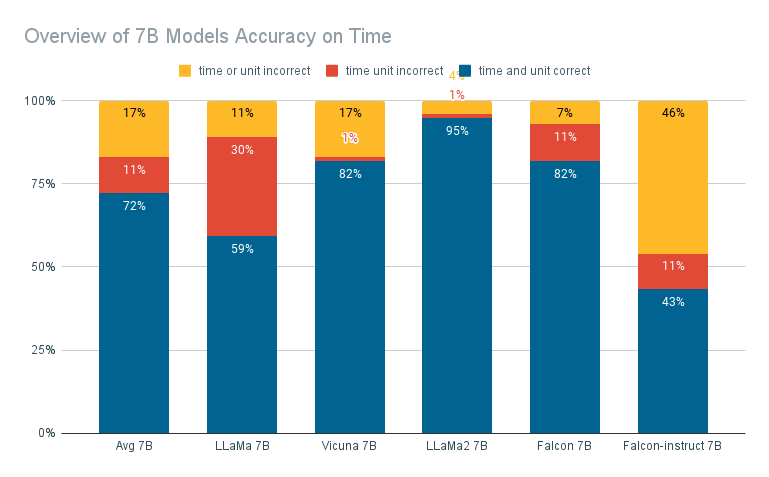
\includegraphics[height=0.7\textheight]{overview_7b_time}
    % \begin{columns}
    %     \column{0.35\textwidth}
    % 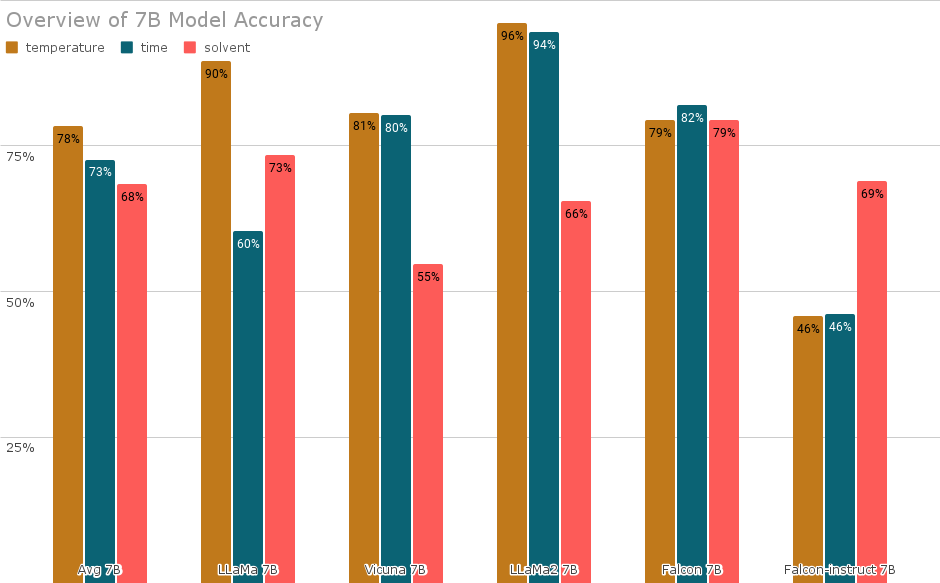
\includegraphics[width=\textwidth]{overview_7b_accuracy}
    % \column{0.65\textwidth}
    % 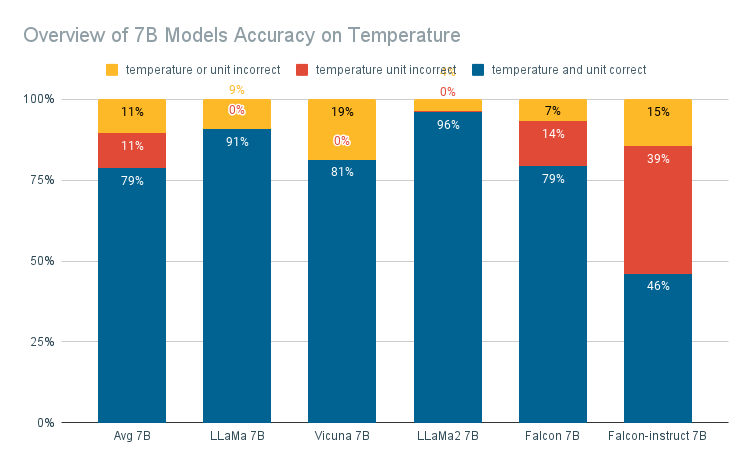
\includegraphics[height=0.7\textheight]{overview_7b_temp}
    % \end{columns}
    % \newpage
    % \begin{columns}
    %     \column{0.35\textwidth}
    % 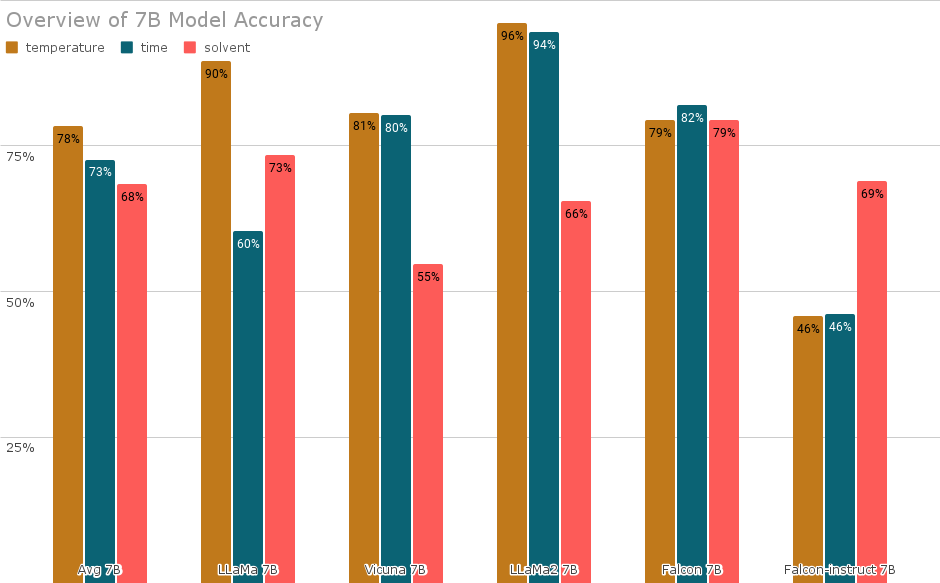
\includegraphics[width=\textwidth]{overview_7b_accuracy}
    % \column{0.65\textwidth}
    % 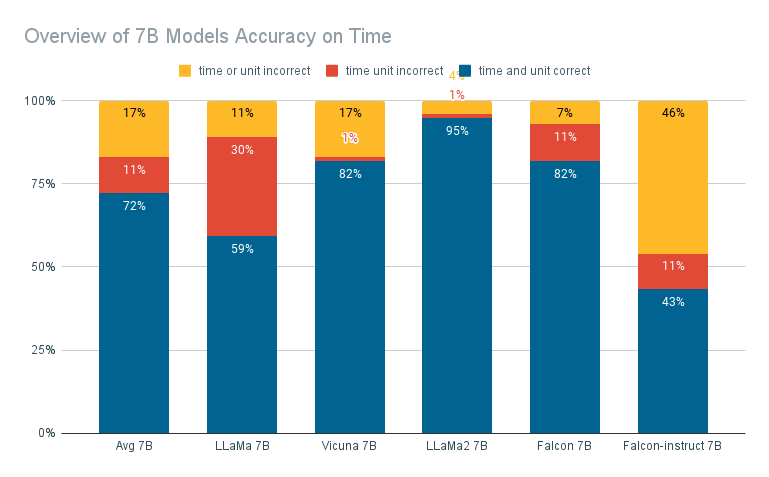
\includegraphics[height=0.7\textheight]{overview_7b_time}
    % \end{columns}
\end{frame}

\begin{frame}<handout>[c]{Note on Unit Confusion}
    \Large 
    \begin{itemize}
        \item Does happen fewer than 0.5\% (0-4 cases) for models sized 13B or more
    \end{itemize}
\end{frame}

\begin{frame}[c,fragile,allowframebreaks]{Solvent Resolution}
    \centering
    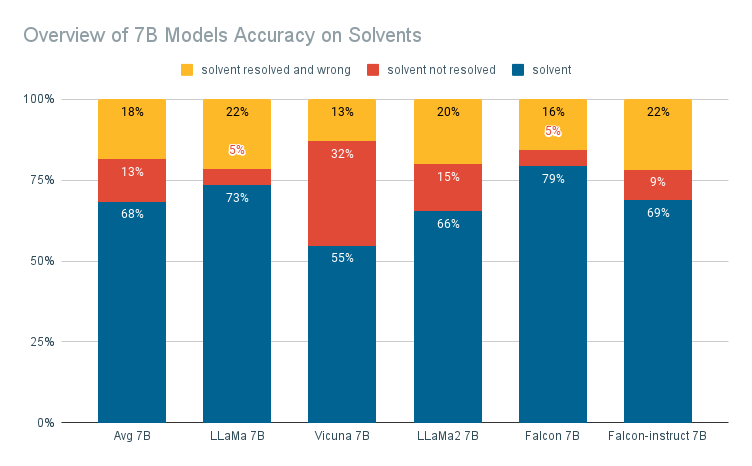
\includegraphics[height=0.7\textheight]{overview_7b_solv}
    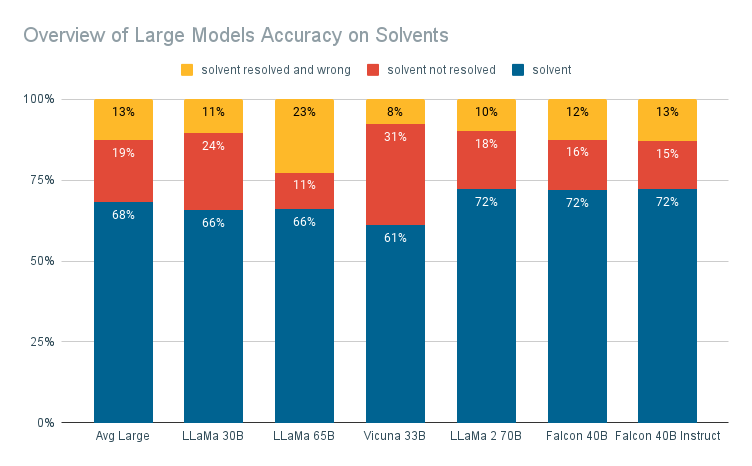
\includegraphics[height=0.7\textheight]{overview_large_solv}
\end{frame}


\begin{frame}[c]{Solvent Resolution?}
    \large
    One hypothesis: Models \textit{are} getting more accurate, but there is a failure in resolving the compounds.

    \vspace{2em}
    \pause

    Remember `distilled H2O'?

    \vspace{2em}
    \pause

    This may be true in particular for the \tsolv \texttt{N,N-DIMETHYLACETAMIDE} (\texttt{cid} 31374), where the synthesis paragraphs contain none of its 125 synonyms in 34 cases (or about 4.37\% of the dataset). 
\end{frame}

\begin{frame}[c]{Fine-Tuning: Excerpt 1}
    \code{input.py}{input}{Excerpt of what could be found in a custom dataloader. \mpy{text} describes any string the model may be provided as input. The tokenizer converts any string to a list of tokens and an attention mask, among other things.\\
    Similar code can be found in tutorials and official sources, e.g. \gls{microsoft} \cite{deepspeedexamples_2023}
}
\end{frame}


\begin{frame}[c]{Fine-Tuning: Failure 1}
    \code{output2.py}{output2}{A model fine-tuned like this returns the following. The \mpy{"} where actually inserted during conversion to \texttt{json} from \texttt{jsonformer}.}
    \only<handout>{
        \large
        Fundamentally, no idea what is going on. It works for others, and it could still be one of many different things that actuatlly happened.
    }
\end{frame}


\begin{frame}[c]{Fine-Tuning: Excerpt 2} 
    \large
    \begin{itemize}[<+(1)->]
        \item Using the \gls{hf} \texttt{trl} (Transformer Reinforcement Learning) library
        \item \mpy{DataCollator} are used for batch-processing inputs
        \item \mpy{DataCollatorForLanguageModeling} abstracting away tokenization, uses \mpy{"text"}-key for training in other examples
        \item Specifically, the example uses \mpy{DataCollatorForCompletionOnlyLM}, deriving from it
    \end{itemize}
\end{frame}


\begin{frame}[c]{Fine-Tuning: Failure 2}
    \code{error.py}{error}{Error when providing \mpy{DataCollatorForCompletionOnlyLM} with a dataloader similar to those in examples.\\Counterintuitively, this is not a \mpy{KeyError}.}
    It also fails when manually tokenizing before the \mpy{DataCollator} (providing tokenized \mpy{"input_ids"} etc. as key, using this or a different \mpy{DataCollator}).
\end{frame}

\chapter{Conclusion}\label{chap:conclusion}
\todo{write conclusion}
\todo{combine scientific question with results}

what was learned, in detail, from the experiments

\chapter{Outlook}\label{chap:outlook}
\todo{outlook chapter guideline: what could be done next? Why was this not done?}
This work aimed to answer numerous questions surrounding the use of \glspl{LLM} for automated data extraction from scientific literature.
The knowledge gained while doing so, allows us to ask more, and better questions.
\todo{write outlook}

\section{More Prompt Engineering}\label{sec:out-prompt}
During this work, a lot of effort was put in attempting to fine-tune the models used (See \secref{sft} for details on \informal{our} work, and \subref{finetune} for details on training and fine-tuning \glspl{LM} in general).
Thus, not much effort was put in getting the most of out prompt engineering.
Better prompts could potentially be automatically generated to work well across models \cite{zhou_large_2022}.
Using tools from mechanistic interpretability \cite{conmy_automated_2023} it should be possible to generate highly-specialized prompts \cite{rumbelow_solidgoldmagikarp_2023} for each model.

% \todo{try duration_in_h and temperature_in_C as prompts}


\informal{We} prompted the model for both

\section{Fine-Tuning}\label{sec:out-sft}
While attempted, \informal{we} where not successfull in fine-tuning one of the selected models (See \secref{sft} for details on \informal{our} work on fine-tuning, and \subref{finetune} for details on training and fine-tuning \glspl{LM} in general).
\todo{expand outlook section on fine-tuning}

\section{Different Frameworks}\label{sub:frameworks}
In recent months a new ecosystem of \gls{LLM} orchestration frameworks emerged.
They are often building on top of the abstraction capabilities of the \acrshort{transformers} library, and bring additional tooling for using \glspl{LLM} for agentic use-cases, but also interfacing, chaining and fine-tuning for various use-cases.
Most prominent for that are currently LangChain \cite{langchain_2023} and HayStack \cite{haystack_2023}, though with the current pace of new frameworks emerging, this may change over time.
A comparison was not done due to time constraints.


\section{Next-Gen Models}\label{sec:next-gen}
Since data extraction for \informal{our} use-case has been established to work with fine-tuning \gls{GPT3} \cite{dunn_structured_2022}, it should in expectation work even better with newer models like \gls{GPT4}.
A comparison was not done due to time and resource constraints.

\section{Comparison to Masked Language Models}\label{sec:masked}
The task of knowledge extraction may be well suited to \glspl{masked} modern \gls{BERT}-derived architectures such as T5 \cite{raffel_exploring_2020}.
A comparison was not done due to time constraints.

% \Appendix

\addchap{Appendix}

\todo{build automated json-to-tables/graphs for all raw values}

% \label{chap:abbr}

% \printglossary[type=\acronymtype, title=List of Abbreviations]


\printglossaries


% \clearpage
% \printglossary[title=List of Abbreviations, toctitle=List of Abbreviations]


% % \addchap{List of Abbreviations, Figures, and Tables}\label{chap:lists}

% \begin{acronym}
%         \acro{ann}[ANN]{Artificial Neural Network}
%         \acro{llm}[LLM]{Large Language Model}
%         \acro{llms}[LLMs]{Large Language Models}
%         \acro{cm}[CM]{Confusion Matrix}
%         \acro{lms}[LMS]{Least Mean Square}
%         \acro{mlp}[MLP]{Multilayer Perceptron}
%         \acro{mof}[MOF]{Metal Organic Framework}
%         \acro{ner}[NER]{Named Entity Recognition}
% \end{acronym}
%
% \begingroup \let\clearpage\relax    % in order to avoid listoffigures and
% % \newpage
% % \listoffigures
% % \newpage
% % \listoftables
% \endgroup
% \cleardoublepage

% \todototoc
\listoftodos

\TheBibliography
\printbibliography[heading=bibintoc]

\end{document}
